\documentclass[letterpaper,11pt]{article}

%-----------------------------------------------------------
\usepackage{latexsym}
\usepackage[empty]{fullpage}
\usepackage[usenames,dvipsnames]{color}
\usepackage{verbatim}
\usepackage[pdftex]{hyperref}
\usepackage{microtype}
\usepackage{graphicx}
\usepackage{multicol}
\hypersetup{
    colorlinks,%
    citecolor=black,%
    filecolor=black,%
    linkcolor=black,%
    urlcolor=mygreylink     % can put red here to visualize the links
}
\urlstyle{same}
\definecolor{mygrey}{gray}{.85}
\definecolor{mygreylink}{gray}{.30}
\textheight=9.0in
\raggedbottom
\raggedright
\setlength{\tabcolsep}{0in}
\renewcommand{\familydefault}{\sfdefault}

% Adjust margins
\addtolength{\oddsidemargin}{-0.375in}
\addtolength{\evensidemargin}{0.375in}
\addtolength{\textwidth}{0.5in}
\addtolength{\topmargin}{-.375in}
\addtolength{\textheight}{0.75in}


%-----------------------------------------------------------
%Custom commands
\newcommand{\resitem}[1]{\item #1 \vspace{-1pt}}
\newcommand{\resheading}[1]{{\large \colorbox{mygrey}{\begin{minipage}{\textwidth}{\textbf{#1 \vphantom{p\^{E}}}}\end{minipage}}}}
\newcommand{\ressubheading}[4]{
\begin{tabular*}{6.5in}{l@{\extracolsep{\fill}}r}
		\textbf{#1} & #2 \\
		\textit{#3} & \textit{#4} \\
\end{tabular*}\vspace{-6pt}}

\newcommand{\ressubheadingleader}[4]{
\begin{tabular*}{6.5in}{l@{\extracolsep{\fill}}r}
		\textbf{#1} & #2 \\
		{#3} & \textit{#4} \\
\end{tabular*}\vspace{-6pt}}





%-----------------------------------------------------------

%-----------------------------------------------------------

%-----------------------------------------------------------

\begin{document}


\begin{comment}		
\begin{figure}[!ht]
	\begin{minipage}[t]{.25\textwidth}
		\vspace{0pt}
    		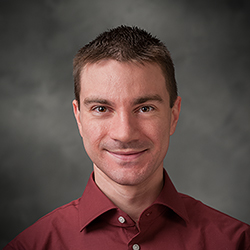
\includegraphics[width=46mm]{Matt-Phinney-64.jpg}
   	 \end{minipage}\hfill
	\begin{minipage}[t]{.72\textwidth}
		\vspace{0pt}
    		\begin{tabular*}{4in}{l@{\extracolsep{\fill}}r}
      			\textbf{{\Huge \textsc{{Matthew D. Phinney}}}} \vspace{0.05in}\\
			{\textbf{{3795 20th Street, San Francisco, CA 94110}}} \vspace{0.05in}\\
			{\textbf{{M.Phinney@GatesScholar.org}}} \vspace{0.05in}\\
			\fbox{\parbox{\textwidth}{I am a Java developer looking to apply my skills to technical, data--driven projects.  My comprehensive knowledge of algorithms and conscientious approach to problem solving allows me to write clean code with superior performance characteristics.  I excel in an environment that fosters creativity and demands polished results, and I look forward to discussing how I might contribute to your team.}}\vspace{0.05in}\\
			%%{\textbf{\href{https://www.linkedin.com/profile/view?id=189910237&trk=nav_responsive_tab_profile}{LinkedIn}}} \vspace{0.05in}\\
			%%{\textbf{\href{https://github.com/MatthewPhinney}{GitHub}}} \vspace{0.05in}\\
    		\end{tabular*}
    	\end{minipage}
\end{figure}
\end{comment}

\renewcommand{\baselinestretch}{1}
 \normalsize

\newcommand{\mywebheader}{
\begin{tabular*}{7in}{l@{\extracolsep{\fill}}r}
	\textbf{{\Huge \textsc{{Matthew D. Phinney}}}}\hfill{\textbf{{M.Phinney@GatesScholar.org}}}\\
	{\textbf{{3795 20th Street, San Francisco, CA 94110}}}\hfill{GitHub: MatthewPhinney} \vspace{0.05in}\\
	\fbox{\parbox{\textwidth}{I am a Java developer looking to apply my skills to technical, data--driven projects.  My comprehensive knowledge of algorithms and conscientious approach to problem solving allows me to write clean code with superior performance characteristics.  I excel in an environment that fosters creativity and demands polished results, and I look forward to discussing how I might contribute to your team.}}\vspace{0.05in}\\
	\end{tabular*}
\\
\vspace{0.15in}}

% CHANGE HEADER SOURCE HERE
\mywebheader

%%%%%%%%%%%%%%%%%%%%%

%%%%%%%%%%%%%%%%%%%%%%
\resheading{\Large{Technical skills}}
\begin{multicols}{2}
	\begin{itemize}
	\large
		\resitem{Java}
		\resitem{C/C++}
		\resitem{Unix command line tools}
		\resitem{GNU Emacs}
		\resitem{Test driven development}
		\resitem{Hudson Continuous Integration}
		\resitem{Git}
		\resitem{Tortoise SVN}
		\resitem{Apache Ant}
		\resitem{Python}
	\end{itemize}
\end{multicols}

\resheading{\Large{Professional Experience}}
\large
	\begin{itemize}
		\item
			\ressubheading{\href{http://www.princeton.com/}{Princeton Consultants}}{Princeton, NJ}{Analyst -- Java development} {October 2012-August 2014}
			
			{ \small
				\begin{itemize}
				\renewcommand{\baselinestretch}{1}
				 \normalsize
					{\resitem{Developed a Java-based web application for an international transportation company}}
					\resitem{Used the Hibernate framework to develop back end Java code to read/write from our SQL database}
					\resitem{Wrote and executed tests with JUnit, following a comprehensive process of test driven development}
					\resitem{Set up Hudson jobs to build source code, run unit tests, and deploy application to WebLogic server}
					\resitem{Used Oracle Coherence to develop a distributed cache for in-memory data storage}
					{\resitem{Used Oracle ADF and JavaScript to develop the UI components of the application}}
					{\resitem{Worked with the business team to deliver, install, and deploy application}}
				\end{itemize}
			}
			
	\end{itemize}




%%%%%%%%%%%%%%%%%%%%%%
\resheading{\Large{Academic Background}}
\large
	\begin{itemize}
		\item
			\ressubheading{\href{http://www.cam.ac.uk/}{Cambridge University}}{Cambridge, UK}{\href{http://www.maths.cam.ac.uk/postgrad/mathiii/}{MASt Pure Mathematics}} {June 2012}
		\item
			\ressubheading{\href{http://www.ox.ac.uk}{Oxford University}}{Oxford, UK}{\href{https://www.maths.ox.ac.uk/members/students/postgraduate-courses/msc-mmsc}{MSc Mathematical Modelling and Scientific Computing}} {September 2011}

			
		\item
			\ressubheading{\href{http://www.trincoll.edu/}{Trinity College}}{Hartford, CT}{{\href{http://www.trincoll.edu/Academics/MajorsAndMinors/Mathematics/Pages/default.aspx}{AB Mathematics,}} {\href{http://www.trincoll.edu/Academics/MajorsAndMinors/Music/Pages/default.aspx}{Music} -- Salutatorian}}{May 2010}

	\end{itemize} 
	
	% End Education list
	
%	\resheading{\Large{Skills}}
%	\begin{itemize}
%	\normalsize		
%		\resitem{Selected Coursework: Stochastic Calculus and Applications, Stochastic Differential Equations, Statistical Theory, C++ for Scientific Computing, Advanced Probability, Numerical Linear Algebra, Numerical Solution of Differential Equations, Finite Element Methods for Partial Differential Equations}
%		\resitem{Computing: Java, Linux/Unix command line, MatLab}
%		
%	\end{itemize}
	
% End coursework list
%%%%%%%%%%%%%%%%%%%%%%
\resheading{\Large{Academic Awards}}
\begin{multicols}{2}
	\begin{itemize}
	\large
		\resitem{\href{http://www.gatescambridge.org/our-scholars/Profile.aspx?ScholarID=5646}{Gates Cambridge Scholar}}
		{ \small
				\begin{itemize}
				\renewcommand{\baselinestretch}{1}
				 \small
					{\resitem{1 of about 40 Americans selected}}
				\end{itemize}
				}
		\resitem{\href{http://www.pbk.org/home/index.aspx}{Phi Beta Kappa}}
				{ \small
				\begin{itemize}
				\renewcommand{\baselinestretch}{1}
				 \small
					{\resitem{National academic honor society}}
				\end{itemize}
		}
		\resitem{\href{http://www.act.org/goldwater/}{Goldwater Scholar}}
		{ \small
				\begin{itemize}
				\renewcommand{\baselinestretch}{1}
				 \small
					{\resitem{1 of about 300 Americans selected}}
				\end{itemize}
		}
		\resitem{\href{http://www.pme-math.org/}{Pi Mu Epsilon}}
						{ \small
				\begin{itemize}
				\renewcommand{\baselinestretch}{1}
				 \small
					{\resitem{National mathematics honor society}}
				\end{itemize}
		}
		\begin{comment}
		\resitem{H. E. Russell Fellowship}
		\resitem{First Prize in First Year Mathematics}
		\end{comment}
	\end{itemize}
\end{multicols}
% End Distinctions list

%\resheading{\Large{Research and Presentations}}
%\begin{itemize}
%\large
%
%	\item
%		\ressubheading{Part III Essay}{Cambridge University}{Deterministic and Stochastic Models for the Multiplicative Coalescent}{2012}
%
%	\item
%		\ressubheading{Part III Seminar}{Cambridge University}{Coagulation with Limited Aggregations}{2012}
%			
%	\item
%		\ressubheading{Part III Seminar}{Cambridge University}{Stochastic Simulation of Chemical Reactions}{2011}
%	
%	\item
%		\ressubheading{MSc Dissertation}{Oxford University}{Multiscale Methods for Stochastic Simulation of Chemical Reactions}{2011}
%
%	\item
%		\ressubheading{Senior Seminar Talk}{Trinity College}{Georg Cantor and the Uncontability of the Reals}{2010}
%				
%	\item
%		\ressubheading{Interdisciplinary Science Program Research Apprenticeship}{Trinity College}{Labeling the Petersen Graph}{2007}
%
%								
%\end{itemize}

%%%%%%%%%%%%%%%%%%%%%%
\begin{comment}
\resheading{\Large{Service Projects}}
\large
	\begin{itemize}
			\item 
			\ressubheading{\href{http://www.odauk.org/}{Oxford Development Abroad}}{Mbale, Uganda}{\href{http://www.littlebigafrica.org/}{Little Big Africa}}{Summer 2009}
				{ \small
				\begin{itemize}
				\renewcommand{\baselinestretch}{1}
				 \normalsize
					{\resitem{Worked with engineers to construct a cistern at a local school}}
					{\resitem{Worked with community members to build smokeless cook-stoves}}

				\end{itemize}
				}
				
%						\item 
%			\ressubheadingleader{{Trinity College Supplemental Instruction Program}}{Trinity College}{Supplemental Instruction Leader in Single Variable Calculus}{Fall 2007}
%			{\small
%			\begin{itemize}
%			\renewcommand{\baselinestretch}{1}
%			\normalsize
%			{\resitem{Led review sessions and assisted in preparing examinations}}
%			 \end{itemize}
%			 }
%			\renewcommand{\baselinestretch}{1}
		\item
			\ressubheading{\href{http://www.davisprojectsforpeace.org/}{Kathryn Wasserman Davis 100 Projects for Peace Grant Winner}}{Kathmandu, Nepal}{\href{http://www.davisprojectsforpeace.org/projects/2007/node/243}{A community approach to solar lighting}}{Summer 2007}
				{ \small
				\begin{itemize}
				\renewcommand{\baselinestretch}{1}
 				\normalsize
					{\resitem{Developed and implemented a self-designed solar energy project}}
					{\resitem{Installed photovoltaic panels in two Nepali villages}}
				\end{itemize}
          			}
		

	\end{itemize}  % End Experience list
	\end{comment}



\end{document}